%%% Local Variables:
%%% mode: latex
%%% TeX-master: t
%%% End:

\chapter{A brief tour of Cloud Haskell }
\label{chap:cloudhaskell}

In this chapter, we will briefly cover the overall design decisions
which influence the development of Cloud Haskell. This is really
important in understanding the trade-offs taken by Cloud Haskell. The
problem of hot code reloading and our implementation in the following
chapters depends on the understanding of these decisions.

\section{The Design Decisions}

\subsection{Erlang Style Concurrency}

The key idea is : Program the cluster as a whole, not individual
nodes. Same program runs on all the nodes. The programmer does not
have to worry about how the individual nodes behave. To implement this
model, Cloud Haskell takes inspiration from the Erlang style of
programming which has been highly successful in the industry. The
design decisions are influenced heavily by the motto: ``If in doubt,
do it the way Erlang does it''.  What does Cloud Haskell bring to the
table?
\begin{description}
\item [Improved tooling and library ecosystem] Compared to Erlang,
  Haskell has a much more mature ecosystem of tools and libraries. The
  package manager of Haskell, Hackage has more than 5000 packages
  covering a variety of domains.
\item [Static vs Dynamic Typing] Haskell's static typing with type
  inference eliminates whole class of bugs at compile time.
\item [Modular Architecture] Erlang is the actor model. The networking
  stack is embedded into the run time of Erlang. It is impossible to
  use Erlang in exotic network protocols such as infiniband, CCI, etc
  Cloud Haskell on the other hand keeps the network stack as a library.
\item [Multiple Concurrency Abstractions] Apart from message passing
  across nodes, individual nodes can still use concurrency primitives
  such as Threads and STM as necessary. In case of high capacity,
  multi-core nodes, it might make better sense to use shared
  concurrency constructs than actor model and Cloud Haskell allows
  that. It encourages right abstraction at the right level. Erlang
  does not provide other concurrency primitives.
\item [A more precise and well-defined semantics] Erlang's semantics
  for does not gurantee message reliabilty. In case of node
  disconnects, Erlang buffers the messages temporarily and then drops
  messages, sacrificing reliability property. Since messages cannot be
  buffered indefinitely, it is difficult to guarantee reliability. Cloud
  Haskell instead provides an explicit reconnect primitive to accept
  intermediate message loss.
\end{description}

\subsection{Library vs Run Time System}

Compared to other approaches where the implementation is tied up with
the RTS, Cloud Haskell is implemented as a Haskell Library.
The advantages are the following :
\begin{description}
\item[Portability] As a library, it can be compiled against Haskell compilers other than
GHC.
\item[Modular] The whole architectural flexibility afforded by Cloud Haskell is
  only possible because it is not tied with the RTS. Various layers of
  the stack can be replaced with alternative
  implementations. Moreover, alternative implementations of Cloud
  Haskell can be developed and the trade offs can be
  easily evaluated.
\item[Contributor Friendly] GHC is a huge codebase and monolithic. Any
  contributions from other open-source developers would be difficult
  due to the high barrier to entry in developing patches for GHC and
  getting those patches accepted.
\item[Speed of Development] GHC releases are bi-yearly. Any small
  improvements in Cloud Haskell would have to wait for six months to
  get to mainstream. As a library, the fixes can be uploaded
  continuously to Hackage without any delay.
\end{description}

\subsection{Modular Architecture}

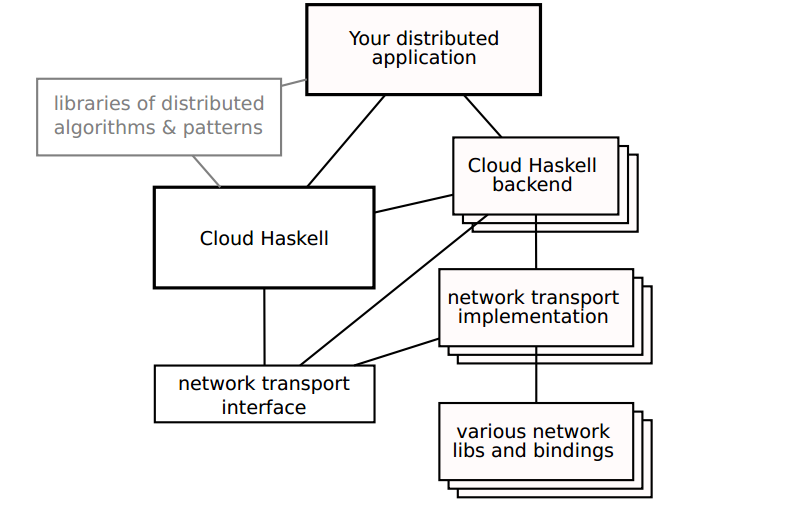
\includegraphics[scale=0.5]{design}

The architecture of Cloud Haskell is highly decoupled from the
transport backend. A major issue with Erlang is that it is difficult
to use in exotic network protocols like infiniband, CCI, etc. Cloud
Haskell has a unified Network Transport interface which provides a
uniform abstraction for a variety of actual network protocols. Porting
a Cloud Haskell program to another network protocol is as simple as
using the corresponding network transport implementation for the given
protocol.  Even the Cloud Haskell module is a stub API which simply
re-exports the actual Cloud Haskell backend API. This makes it very
easy to try out competing implementations of Cloud Haskell itself.

\subsection{The Actor Model and Cloud Haskell}

The dominant model of programming a distributed application running in
a cluster of nodes is via message-passing. MPI cite and Actor
Model cite are the popular models for message-passing. In actor
model, isolated (no shared memory) lightweight processes are the
smallest program primitives. These processes communicate only by
sending and receiving messages.

\subsection{Actor vs Thread}

Although, Actor is a concurrency abstraction similar to Thread, it has
subtle differences which makes it suitable in a distributed setting. A
comparison is listed in the table below.

Actor	Thread
can create more actors	can create more threads
can have private local state	can have private local state
has NO shared state (isolated from other actors!)	has limited shared state
communicates with other actors via asynchronous message passing	communicates with other threads via shared variables

The essential difference between the two is about isolation and
message passing. The appeal of actor model is its simplicity. By
avoiding shared state, it eliminates a whole class of concurrency bugs
by definition. It is easier to reason about because each actor can now
be reasoned about in isolation and independent of other actors.

More formally, an actor is a computational entity that, in response to a
message it receives, can concurrently :
\begin{itemize}
\item send a finite number of messages to other actors
\item create a finite number of new actors
\item designate the behavior to be used for the next message it receives
\end{itemize}

The only popular programming language based on actor model is Erlang.
Recently there has been a rise in the number of different
implementations of actor model. Instead of designing a new programming
language, the current actor based systems are implemented by embedding
as a concurrency paradigm inside a host language. This has obvious
advantages which are discussed in {cite}. Some popular
implementations are Akka (Scala and Java), Celluloid (Ruby) and Cloud
Haskell (Haskell).

\section{The Core API}

For complete documentation of Cloud Haskell API, the haddock
documentation can be read at {cite}.

The central abstraction in Cloud Haskell for message passing is the
Process monad. It keeps track of the state associated with a process,
primarily the message queue associated with the process. Any code
running in the Process monad has access to the data structures
representing the process and can pass these data structures to other
Process-monadic functions that it calls. All functions dealing with
sending and receiving of messages, spawning and linking processes must
be in the Process monad.

Since Process monad in an instance of MonadIO, arbitrary IO functions
can be called in Process monad via liftIO.

ProcessId is a type corresponding to the process identifier. NodeId is
similarly for nodes.

Any type which is an instance of Typeable and Binary is also an
instance of Serializable.

send takes a process-id and a serializable message and sends it
asynchronously to the corresponding process.
An example in the next section demonstrates the send and receive
functions.

\begin{program}

\caption[Cloud Haskell API]
{Core API}

\label{fig:cloud-haskell-api}
\begin{minted}{haskell}

instance Monad Process
instance MonadIO Process

data ProcessId
data NodeId

class (Typeable a, Binary a) => Serializable a

send :: Serializable a => ProcessId -> a -> Process ()
expect :: Serializable a => Process a

spawn :: NodeId -> Closure (Process ()) -> Process ProcessId

getSelfPid :: Process ProcessId
getSelfNode :: Process NodeId

\end{minted}
\end{program}


\section{Ping Pong in Cloud Haskell}

\begin{program}

\caption[Ping Pong in Cloud Haskell]
{Ping Pong in Cloud Haskell}

\label{fig:ping-pong-intro}
\begin{minted}{haskell}

module Main where
import Control.Concurrent ( threadDelay )
import Data.Binary
import Data.Typeable
import Control.Distributed.Process
import Control.Distributed.Process.Node
import Network.Transport.TCP

data Ping = Ping deriving (Typeable)
-- binary instance declaration of Ping
instance Binary Ping where
    put Ping = putWord8 0
    get      = do { getWord8; return Ping }
-- Ping is now serializable
server rPing = do
    Ping <- receiveChan rPing
    liftIO $ putStrLn "Got a ping!"

client :: SendPort Ping -> Process ()
client sPing =
    sendChan sPing Ping

ignition :: Process ()
ignition = do
    -- start the server
    sPing <- spawnChannelLocal server
    -- start the client
    spawnLocal $ client sPing
    liftIO $ threadDelay 100000 -- wait a while

main :: IO ()
main = do
    Right transport <- createTransport "127.0.0.1" "8080"
                            defaultTCPParameters
    node <- newLocalNode transport initRemoteTable
    runProcess node ignition

\end{minted}
\end{program}

This program is the hello world equivalent in distributed systems. A
client process sends a Ping to the server process. On receiving the
Ping, the server process prints a message ``Got a Ping''.

In main, we initialize a network transport tcp backend, setup a local
node and run the process ``ignition'' on the local node.

The process ``ignition'' spawn the ``server'' process and the
``client'' process on the local node and waits a while otherwise the
child processes will get killed when the parent terminates.

A channel is a tuple (SendPort a, ReceivePort a) on which only values
of type ``a'' can be transmitted. In this case, it is the data type
Ping. We create a binary instance of Ping to make it serializable.

The client sends Ping on the SendPort of server. In case of server,
receiveChan blocks until a message of type Ping is received on the
receive port. On receiving the message, server prints ``Got a Ping''
to the console.